\documentclass[11pt, oneside]{article}   	% use "amsart" instead of "article" for AMSLaTeX format
\usepackage{geometry}                		% See geometry.pdf to learn the layout options. There are lots.
\geometry{letterpaper}                   		% ... or a4paper or a5paper or ... 
%\geometry{landscape}                		% Activate for for rotated page geometry
%\usepackage[parfill]{parskip}    		% Activate to begin paragraphs with an empty line rather than an indent
\usepackage{graphicx}				% Use pdf, png, jpg, or eps� with pdflatex; use eps in DVI mode
								% TeX will automatically convert eps --> pdf in pdflatex		
\usepackage{amssymb}
\usepackage{amsmath}
\usepackage{parskip}
\usepackage{color}

\title{Average value of a function}
%\author{The Author}
%\section{}
% \subsection*{R code}
\date{}							% Activate to display a given date or no date

\graphicspath{{/Users/telliott_admin/Dropbox/Tex/png/}}

% \begin{center} 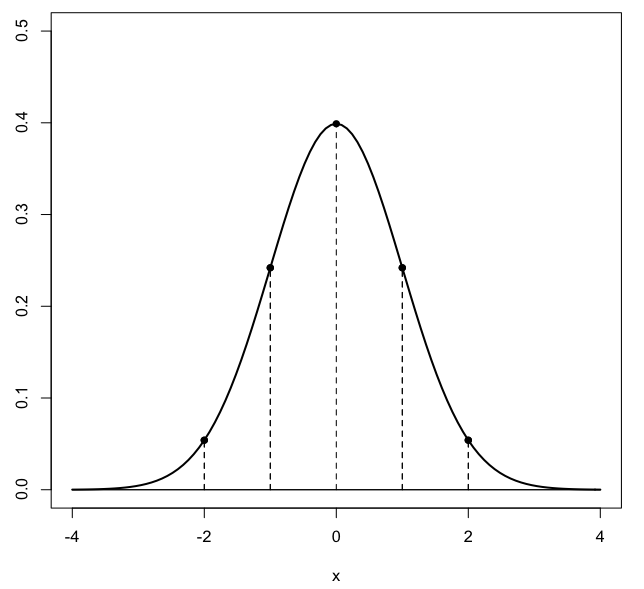
\includegraphics [scale=0.4] {gauss3.png} \end{center}

\begin{document}
\maketitle
\Large
\noindent

We want to consider the idea of the \emph{average value} of a function (over an interval).  One way to think of that would be, by analogy to a list of numbers, to collect the values of $f(x)$ at each point along the graph of the function, and then obtain the mean.  Of course, the fact that there are an infinite number of such points is a bit of an issue.

Let's think of it another way.  Suppose we integrate and find the total area under the curve between $x=a \rightarrow b$.  Take the number calculated from the definite integral, divide by the distance $b-a$, and plot the result as a height $h$ so as to form a rectangle above the $x-axis$.

\begin{center} 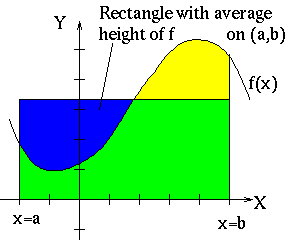
\includegraphics [scale=0.6] {avgvalue.png} \end{center}

Clearly $h$ is a reasonable stand-in for the average value of $f(x)$, since the rectangle formed from $ [a,b] \times [0,h]$ gives the same area as we found under the curve by integration.  Call this $\bar{f}(x)$.  Define it to be

\[ \bar{f}(x) = \frac{1}{b-a} \int_a^b f(x) \ dx \]

The average value of a function over an interval is the integral of the function divided by the length of the interval.

This definition also works in 2D or more dimensions.  Consider the unit circle centered at the origin.  We compute the average value of $x$:

\[ \bar{x} = \frac{1}{Area} \ \iint_R x \ dA \]

where the area is, of course, the same integral but without the function $x$ inside.

Since we do have the $x$, we might want to keep Cartesian coordinates.  The limits on $y$ are the usual ones.  We set it up like so:

\[ \int_{x=-1}^{1} \int_{y=-\sqrt{1-x^2}}^{\sqrt{1-x^2}} x \ dy \ dx \]

The inner integral is just

\[ xy \ \bigg |_{y=-\sqrt{1-x^2}}^{\sqrt{1-x^2}} \]
\[ = 2 x \sqrt{1-x^2} \]

And the outer integral is

\[ \int_{x=-1}^{1} 2 x \sqrt{1-x^2} \ dx \]
\[ = -(1-x^2)^{3/2} \ \bigg |_{-1}^1 = 0 \]

The area is $\pi$ but zero times $1/\pi$ is still zero.  And I suppose it is not a surprise that the average value of $x$ over a circle centered at $0$ is just $0$.

The reason I bring this up is a problem in Varberg that has an easy solution and a hard solution.  We've done part of the easy solution here, and the reason I know this is Auroux shows the answer.  Varberg does only the hard calculation, which is a little weird.

\begin{center} 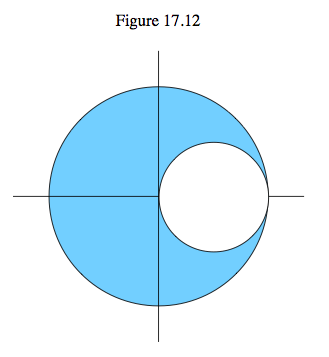
\includegraphics [scale=0.6] {Varberg17-12.png} \end{center}

The diagram shows the unit circle at the origin in blue with an inset missing circle in white.  The missing circle has radius $1/2$ and is centered at $1/2,0$.  The problem is to find the average value of the function $x$ over the blue region.

Now, we've just finished showing that the average value of $x$ over the unit circle is zero.  But $\bar{x}$ over the small circle will not be zero, and we will obtain minus that value by subtracting from the big circle.  

\[ \bar{x} = \frac{1}{Area} \ \iint_R x \ dA \]

Surely $\bar{x}$ over the small circle is $1/2$, multiplied by the area $\pi/4$ and negated because of the subtraction, we predict the answer will be $- \pi/8$.

Let's try to do the problem the way its done in Varberg.

The idea is to use polar coordinates.  It's really hard to see how you could possibly do it in Cartesian coordinates, except in the way that we already used them.  How do we describe the $x$-dependence of the bounds on $y$?  I suppose we could try, but lets go with polar.  We will integrate the top half of the circle, and we'll do it separately for the first and second quadrants.

\[ \int \int x \ r \ dr \ d \theta \]
\[ x = r \cos \theta \]
\[ \int \int r \cos \theta \ r \ dr \ d \theta \]

Pretty standard.  We will integrate with respect to $\theta$ last.  So, now our job is to figure out how what the lower limit is on $r$ as $\theta$ varies.  And I don't know how you would see it if you didn't know the answer, but it is just $\cos \theta$.  

We can check that this gives the correct lower limit on $r$ for the two extremes $\theta = 0$ and $\theta = \pi/2$.  We'll come back to the issue of how this was found later.  Let's calculate:

\[ \int_0^{\pi/2} \int_{\cos \theta}^{1} r \cos \theta \ r \ dr \ d \theta \]

The inner integral is

\[ \frac{r^3}{3} \cos \theta \ \bigg |_{\cos \theta}^{1} \]

So the outer integral is then

\[ \frac{1}{3} \int_0^{\pi/2} \cos \theta - \cos^4 \theta  \ d \theta \]

So we will have an outside factor of $1/3$ and $\sin \theta$ between $0$ and $\pi/2$, which is just 1, but we have to deal with the fourth power of the cosine.  Yecch...  Recall the double-angle formula:

\[ \cos^2 s = \frac{1}{2} (1 + \cos 2s) \]
\[ \cos^4 s = \frac{1}{4} (1 + \cos 2s)^2 \]
\[ = \frac{1}{4} (1 + 2 \cos 2s + \cos^2 2s) \]

Substitute $t = 2s$
\[ \cos^2 2s = \cos^2 t = \frac{1}{2} (1 + \cos 2t) \]
\[ = \frac{1}{2} (1 + \cos 4s) \]
Substitute back to the previous version

\[ \frac{1}{4} (1 + 2 \cos 2s + \cos^2 2s) \]
\[ = \frac{1}{4} (1 + 2 \cos 2s + \frac{1}{2} (1 + \cos 4s)) \]

Rearrange slightly

\[ = \frac{3}{8} + \frac{1}{2} \cos 2s + \frac{1}{8} \cos 4s \]

Substitute $\theta$, integrate and get 

\[ = \frac{3}{8}\theta + \sin 2 \theta + \frac{1}{2} \sin 4 \theta \]

With limits of $\theta = 0 \rightarrow \pi/2$ we have only the first term and that one only at the upper limit

\[  = \frac{3}{16} \pi \]

Combine it with the rest of the integral to obtain

\[ \frac{1}{3}(1 - \frac{3}{16} \pi ) \]

Now, on to the second quadrant.

\[ \int_{\pi/2}^{\pi} \int_{0}^{1} r \cos \theta \ r \ dr \ d \theta \]

The inner integral is 

\[ \frac{1}{3} r^3 \cos \theta \ \bigg |_0^1  \]
\[ = \frac{1}{3} \cos \theta \]

And the outer integral is then

\[   \frac{1}{3}  \int_{\pi/2}^{\pi} \cos \theta \ d \theta \]

which is just $-1/3$.  So finally, we add them up:

\[ \frac{1}{3}(1 - \frac{3}{16} \pi ) - \frac{1}{3} = - \frac{\pi}{16} \]

Recall that we integrated only the top half of the figure, so multiply by $2$ to obtain the same answer that we had much more simply before!

\subsection*{Insight}

The part I like about this problem is seeing the limits on $r$.  Varberg do not give a clue about this.  

The equation of a circle in polar coordinates is given as

\[ r = a \cos \theta + b \sin \theta \]

where $(a/2,b/2)$ is the center of the circle.  Thus our small circle has the equation

\[ r = \cos \theta \]

How to check that?  Well, we can convert from polar to Cartesian like this:

\[ x = r \cos \theta \]
\[ x = r^2 = x^2 + y^2 \]
\[ x^2 - x + y^2 = 0 \]

Complete the square:

\[ x^2 - x + \frac{1}{4} + y^2 = \frac{1}{4} \]
\[ (x - \frac{1}{2})^2 + y^2 = \frac{1}{4} \]

This is indeed our circle.

So we can think of this as having $\theta$ in sync for the two circles.  As we advance the parameter for the large circle, we can find the position of $r$ (where the point is with respect to the origin), at the same value of $\theta$ for the small circle.  At least, that's how it seems to me.

We have to remember that for an off-center circle (not at the origin) in polar coordinates the $r$ parameter is still with respect to the origin, rather than with respect to the center of the circle.

\end{document}  